% =========================================================================
% Capítulo 5 — O Benchmark Multicritério (AI-1)
%
% Fontes da verdade: latex/ai1/main.tex (formulação auditada, out/2026 —
% prevalece), dissertation/cap5-benchmark.md (prosa v1),
% notebooks/TABELA_RESULTADOS.md (tabela mestra).
%
% FIGURAS USADAS (copiar para dissertacao/images/):
%   cd_diagram_binary.pdf      <- latex/ai1/figures/cd_diagram_binary.pdf
%   pareto_binary.pdf          <- latex/ai1/figures/pareto_binary.pdf
%   learning_curves.pdf        <- latex/ai1/figures/learning_curves.pdf
%   average_ranks.pdf          <- latex/ai1/figures/average_ranks.pdf
%   dataset_landscape.pdf      <- results/figures/dataset_landscape.pdf
%   heatmap_classification.pdf <- results/figures/heatmap_classification.pdf
%   inference_time.pdf         <- results/figures/inference_time.pdf
%   imbalance_robustness.png   <- results/figures/imbalance_robustness.png
% =========================================================================

\chapter{O Benchmark Multicritério}
\label{chap:benchmark}

\begin{resumocapitulo}
Este capítulo apresenta os resultados do benchmark de 14 modelos
tabulares sobre 18 conjuntos de dados do OpenML (250 das 252 células
possíveis; duas exclusões estruturais), executado sob o protocolo único do
Capítulo~\ref{chap:metodologia}. A leitura tem dois movimentos. Primeiro,
restrito ao núcleo de 11 modelos do estudo (os modelos anteriores à
extensão de 2026 do benchmark), o topo da acurácia é um empate
estatístico --- 8 dos 10 modelos não-líderes são praticamente
equivalentes ao líder sob uma região de equivalência prática (ROPE) de
$\pm$0,01 de AUC --- e 80\% da variância de rank é intrafamília
($\eta^2 = 0{,}20$): o modelo específico importa mais que a família, e a
decisão migra para custo, latência, robustez e estrutura da tarefa.
Segundo, a geração 2026 quebra o empate: o TabFM, \emph{zero-shot},
lidera o rank médio nas três tarefas e é o melhor modelo em 13 dos 18
conjuntos --- ao custo de quatro a cinco ordens de magnitude em latência
de inferência (43.262 vs.\ 0,33~\us/linha no \texttt{adult}). Como
resultados complementares, o capítulo registra o teste independente
desfavorável da família Kolmogorov--Arnold (KAN e TabKAN no último terço
nas três tarefas) e as reversões condicionais que alimentam o arcabouço
de decisão do Capítulo~\ref{chap:framework}.
\end{resumocapitulo}

\publicacaoassociada{Este capítulo corresponde ao primeiro trabalho
individual do programa (AI-1), cuja versão em formato de artigo está em
\texttt{latex/ai1/} no repositório do estudo. Todo número citado aqui
rastreia a um artefato versionado; os caminhos estão registrados em
comentários na fonte \LaTeX{} do artigo e na tabela mestra
(\texttt{notebooks/TABELA\_RESULTADOS.md}).}

O capítulo aplica os instrumentos estatísticos apresentados na
Fundamentação (Capítulo~\ref{chap:fundamentacao}) às estimativas
produzidas pelo protocolo experimental do
Capítulo~\ref{chap:metodologia}, e organiza a evidência em quatro atos.
A Seção~\ref{sec:cap5-cobertura} delimita a cobertura do benchmark e o
roteiro da exposição. O Ato~I (Seção~\ref{sec:cap5-ato1}) estabelece o
empate estatístico do núcleo de 11 modelos e disseca sua anatomia; o
Ato~II (Seção~\ref{sec:cap5-ato2}) mostra que os modelos empatados em
acurácia diferem em ordens de magnitude nos eixos de custo; o Ato~III
(Seção~\ref{sec:cap5-ato3}) mapeia as reversões condicionais --- quando a
estrutura do problema muda o vencedor --- e o eixo do tamanho amostral; o
Ato~IV (Seção~\ref{sec:cap5-ato4}) registra a quebra do empate pela
geração 2026 e o resultado negativo das redes de Kolmogorov--Arnold. A
Seção~\ref{sec:cap5-sintese} encadeia os três fatos que motivam os dois
capítulos seguintes.

\section{Cobertura e organização da evidência}
\label{sec:cap5-cobertura}

O benchmark completa \textbf{250 das 252 células} possíveis (14 modelos
$\times$ 18 conjuntos de dados). As duas ausências são exclusões
estruturais documentadas, não falhas de execução: o conjunto
\texttt{helena}, com 100 classes, excede o limite arquitetural de classes
dos dois \emph{foundation models} (TabPFN e TabFM), que portanto não
produzem predição nele. Essa distinção importa para a leitura
estatística: células ausentes por limite arquitetural são informação
sobre o modelo --- um critério de decisão em si, retomado no
Capítulo~\ref{chap:framework} --- e não dados faltantes a imputar.
Registre-se também que o episódio de retificação de rótulo descrito no
Capítulo~\ref{chap:metodologia} (o conjunto historicamente chamado
``diamonds'' é, na verdade, o \texttt{kin8nm}) precede todos os números
reportados neste capítulo: cada valor aqui citado é posterior à errata.

Antes dos resultados, convém revisitar o espaço amostral sobre o qual
eles se apoiam. A Figura~4.1, no Capítulo~\ref{chap:metodologia},
posiciona os 18 conjuntos no plano amostras $\times$ atributos;
retomamos aqui apenas a leitura de que este capítulo precisa. Ela mostra
que a amostra de conjuntos não se concentra em um único
regime: há conjuntos pequenos e grandes, estreitos e largos, nas três
tarefas --- condição necessária para que as análises condicionais do
Ato~III (desbalanceamento, cardinalidade categórica, tamanho) tenham
variação a explorar. A ressalva simétrica também fica visível: com 10
conjuntos binários, 3 multiclasse e 5 de regressão, o poder estatístico
por tarefa é limitado, e o texto declara essa limitação em cada ponto em
que ela é vinculante.

\paragraph{O núcleo de 11 modelos e a extensão de 2026.}
Ao longo do capítulo, duas grades de comparação coexistem e precisam ser
distinguidas desde já. O \emph{núcleo de 11 modelos} do estudo reúne os
modelos anteriores à extensão de 2026 do benchmark: os três GBDTs
(XGBoost, LightGBM, CatBoost), sete modelos de aprendizado profundo (MLP,
FT-Transformer, SAINT, TabNet, STab, RealMLP, TabM) e um \emph{foundation model}
(TabPFN). A \emph{grade completa de 14} acrescenta os três modelos
incorporados na extensão: o \emph{foundation model} TabFM
\citep{tabfm2026,kong2026} e as duas redes de Kolmogorov--Arnold (KAN
\citep{kan2024} e TabKAN \citep{tabkan2025}). Os Atos~I a III leem o
núcleo de 11 --- é sobre ele que a máxima ``\emph{boosting} sempre
vence'' \citep{grinsztajn2022,mcelfresh2023} foi formulada e é sobre ele
que o empate se estabelece; o Ato~IV lê a grade completa e mostra o que a
extensão muda.

\paragraph{O protocolo em uma frase (e suas assimetrias declaradas).}
Para a leitura autocontida deste capítulo, vale recapitular o essencial
do Capítulo~\ref{chap:metodologia}: validação cruzada aninhada ($5$
folds externos $\times$ $3$ internos, com hiperparâmetros selecionados
apenas nos internos), ajuste bayesiano via Optuna/TPE \citep{akiba2019}
com orçamento equalizado por família (100 tentativas para GBDTs, 25 para
DL), \emph{hold-out} fixo de 20\% (semente 42) que nenhuma etapa de seleção
jamais observa, e pré-processamento por família (one-hot para atenção,
ordinal para árvores, embeddings onde o modelo os define). Duas
assimetrias do desenho são declaradas porque afetam a leitura dos
resultados: os orçamentos de 100/25 tentativas equalizam o custo de
relógio do ajuste (uma tentativa de DL custa aproximadamente
$4\times$ uma de GBDT), e os \emph{foundation models} entram
\emph{zero-shot} --- sem ajuste algum --- porque essa entrada é a
própria alegação de paradigma sob teste; suas configurações de
inferência (\emph{ensemble} de 8 membros, teto de contexto de 50 mil linhas)
são políticas fixas de biblioteca, não quantidades ajustadas aos nossos
dados.

\section{Ato I --- o empate estatístico do núcleo de 11 modelos}
\label{sec:cap5-ato1}

\paragraph{O teste global rejeita a igualdade; o \emph{post-hoc} não
separa o topo.}
Restrita ao núcleo de 11 modelos, a classificação binária ($N{=}10$
conjuntos) exibe um topo estatisticamente indistinguível. O teste
omnibus rejeita a igualdade global de ranks (Friedman
$\chi^2 = 31{,}3$, $p = 5{,}2\times10^{-4}$; correção de Iman--Davenport
$F = 4{,}1$, $p = 1{,}1\times10^{-4}$) --- há, portanto, diferenças reais
em algum lugar da grade --- mas o post-hoc de Nemenyi
\citep{demsar2006} não separa o pelotão superior: os modelos do topo
caem dentro de uma mesma distância crítica. A
Figura~\ref{fig:cap5-cd} apresenta o diagrama de distância crítica, o
instrumento visual canônico dessa análise, aqui exibido já sobre a grade
completa de 14 modelos para evitar duplicação de figura; as estatísticas
do Ato~I são computadas sobre a restrição aos 11, cuja ordem relativa o
diagrama preserva.

\begin{figure}[htbp]
\centering
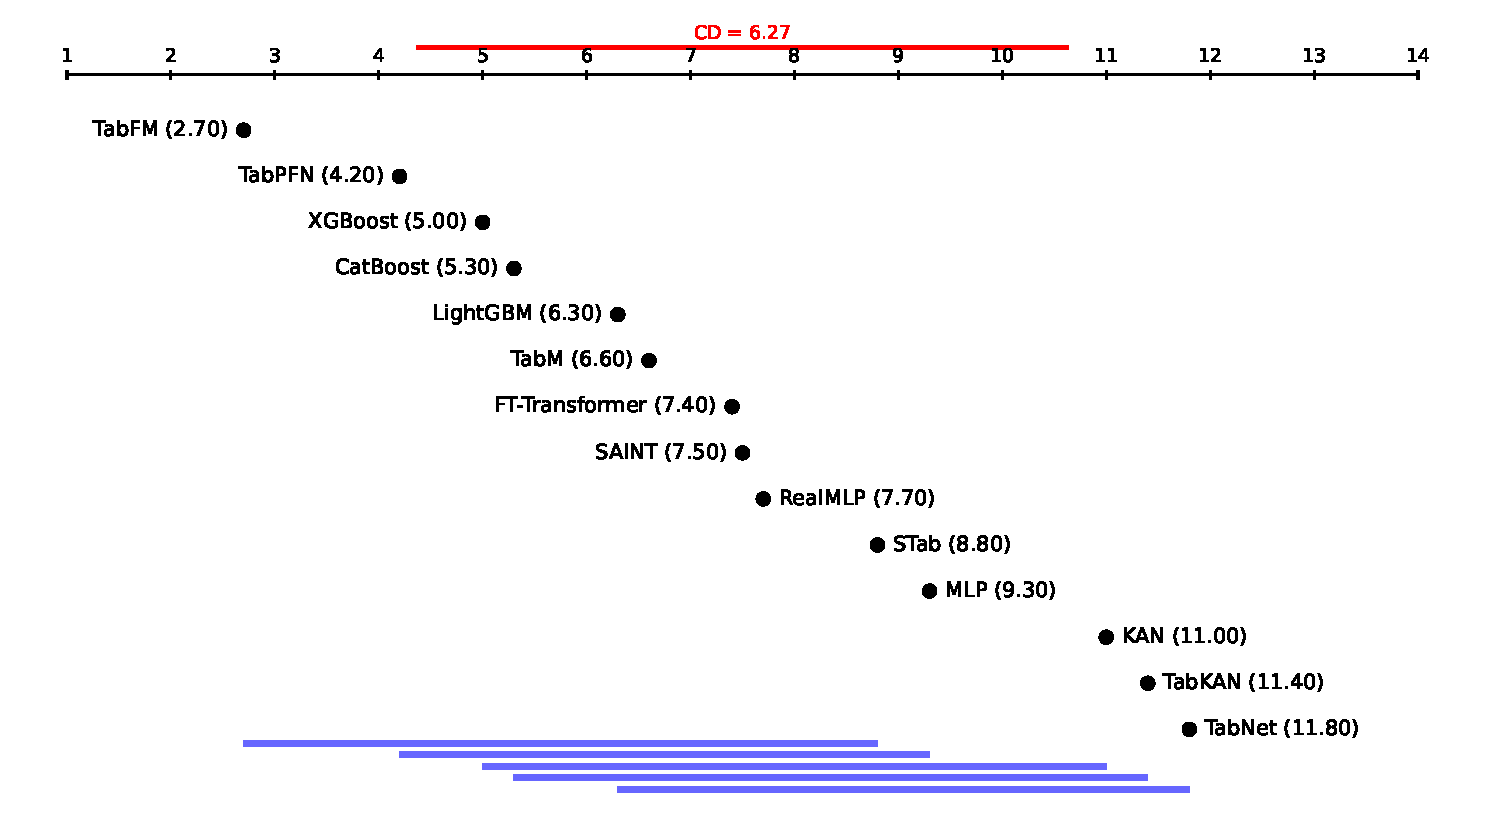
\includegraphics[width=0.9\linewidth]{images/cd_diagram_binary.pdf}
\caption[Diagrama de distância crítica (Nemenyi) --- classificação
binária]{\textbf{O post-hoc não separa o pelotão superior: as barras
horizontais conectam grupos estatisticamente inseparáveis, e elas são
largas.} Diagrama de distância crítica (Nemenyi) para a classificação
binária, todos os 14 modelos ($N{=}10$ conjuntos, CD $= 6{,}27$). O eixo
é o rank médio (menor é melhor); modelos a uma distância menor que a
barra CD não são estatisticamente separáveis, e cada barra horizontal na
parte inferior conecta um grupo inseparável --- a largura dessas barras é
a forma visual da cautela sobre o CD largo discutida na
Seção~\ref{sec:cap5-ato4}. As estatísticas do Ato~I no texto restringem-se
ao núcleo de 11 modelos. Rótulos internos da figura em inglês e decimais com ponto (figura canônica do \emph{benchmark}); eixos e leitura descritos nesta legenda. Fonte:
\texttt{latex/ai1/figures/cd\_diagram\_binary.pdf}.}
\label{fig:cap5-cd}
\end{figure}

A interpretação exige a ressalva imediata: um post-hoc que não separa
não é, por si só, evidência de equivalência --- com $k$ grande e $N$
pequeno, a distância crítica é larga por construção, e ``não separável''
pode significar apenas ``sem poder para separar''. É exatamente por isso
que o protocolo pré-registrou instrumentos mais finos, apresentados no
Capítulo~\ref{chap:fundamentacao} e aplicados a seguir.

\paragraph{A leitura bayesiana: equivalência prática, não ausência de
poder.}
O teste bayesiano \emph{signed-rank} com região de equivalência prática
(ROPE) \citep{benavoli2017} responde à pergunta que o frequentista não
alcança: qual a probabilidade de a diferença entre dois modelos ser
\emph{praticamente irrelevante}? Com ROPE de $\pm$0,01 de AUC, o teste
declara \textbf{8 dos 10} modelos não-líderes praticamente equivalentes
ao líder de rank do núcleo (TabPFN). A análise de sensibilidade do
limiar --- pré-registrada precisamente para evitar que a conclusão
dependa de uma escolha arbitrária --- mostra a progressão
$0{,}005/0{,}01/0{,}02 \to 2/8/10$ equivalentes: a conclusão de empate
vale na margem de um ponto percentual de AUC. Lendo massa posterior
acima de 0,5 como ``mais provavelmente equivalente que não'', o XGBoost
($P(\mathrm{equiv}) = 0{,}65$) supera essa barra mesmo no limiar
estrito de 0,005, com o CatBoost no limite (0,54). O empate do topo,
portanto, não é um artefato de baixo poder: é equivalência prática
positivamente aferida.

\achado{5.1}{No núcleo de 11 modelos, o topo da classificação binária é um
empate estatístico: 8 dos 10 modelos não-líderes são praticamente
equivalentes ao líder sob ROPE de $\pm$0,01 de AUC, e a conclusão
sobrevive à variação do limiar.}
O omnibus rejeita a igualdade global, mas o post-hoc não separa o
pelotão superior e o instrumento bayesiano declara equivalência prática
--- a máxima ``boosting sempre vence'' não encontra, nessa geração,
margem de acurácia que a sustente.

\paragraph{O escopo do empate: onde há poder para afirmá-lo.}
Uma delimitação honesta antes de prosseguir: o empate é estabelecido na
classificação binária, a única tarefa com $N$ suficiente ($N{=}10$) para
que os instrumentos operem com poder útil. Na regressão, $N{=}5$ impõe
um piso combinatório ao p-valor do teste de Wilcoxon pareado (0,0625 ---
nenhuma comparação pode cruzar o limiar convencional de 5\% ali, por
aritmética, não por ausência de efeito); na multiclasse, $N{=}3$ reduz
qualquer análise ao plano descritivo. Essas limitações são declaradas em
cada seção em que se tornam vinculantes, e nenhum achado numerado deste
capítulo depende de significância em tarefa sem poder para aferi-la.

\paragraph{A anatomia do empate: a família é uma abstração fraca.}
Se o topo empata, resta perguntar o que, afinal, explica a variação de
desempenho que existe. A decomposição de variância de ranks por família
responde: $\eta^2 = 0{,}20$ --- apenas 20\% da variância de rank é
explicada pelo pertencimento à família (GBDT, DL, \emph{foundation model}), e
\textbf{80\% é intrafamília}. ``GBDT vs.\ DL'', o eixo em torno do qual a
literatura organizou a década, é uma abstração fraca para esses dados: o
modelo específico importa mais que a família a que pertence. Uma
ressalva de leitura acompanha o número: com as famílias desbalanceadas do
núcleo (3 GBDTs, 7 DL, 1 \emph{foundation model}), essa partição é mecanicamente
conservadora --- ainda assim, a ordem de grandeza da razão
intra/entre-famílias sustenta a conclusão qualitativa.

\achado{5.2}{Oitenta por cento da variância de rank é intrafamília
($\eta^2 = 0{,}20$): escolher bem o modelo dentro da família importa mais
do que escolher a família.}
Esse achado reorienta a pergunta prática de ``qual família?'' para ``qual
modelo, sob quais restrições?'' --- a semente do arcabouço do
Capítulo~\ref{chap:framework}.

\paragraph{O que o agregado esconde: a visão por conjunto.}
O diagrama de distância crítica e o $\eta^2$ operam sobre ranks
agregados; nenhum dos dois mostra as magnitudes absolutas nem onde,
conjunto a conjunto, as diferenças moram. A
Figura~\ref{fig:cap5-heatmap} complementa essa lacuna com o mapa de calor
da classificação.

\begin{figure}[htbp]
\centering
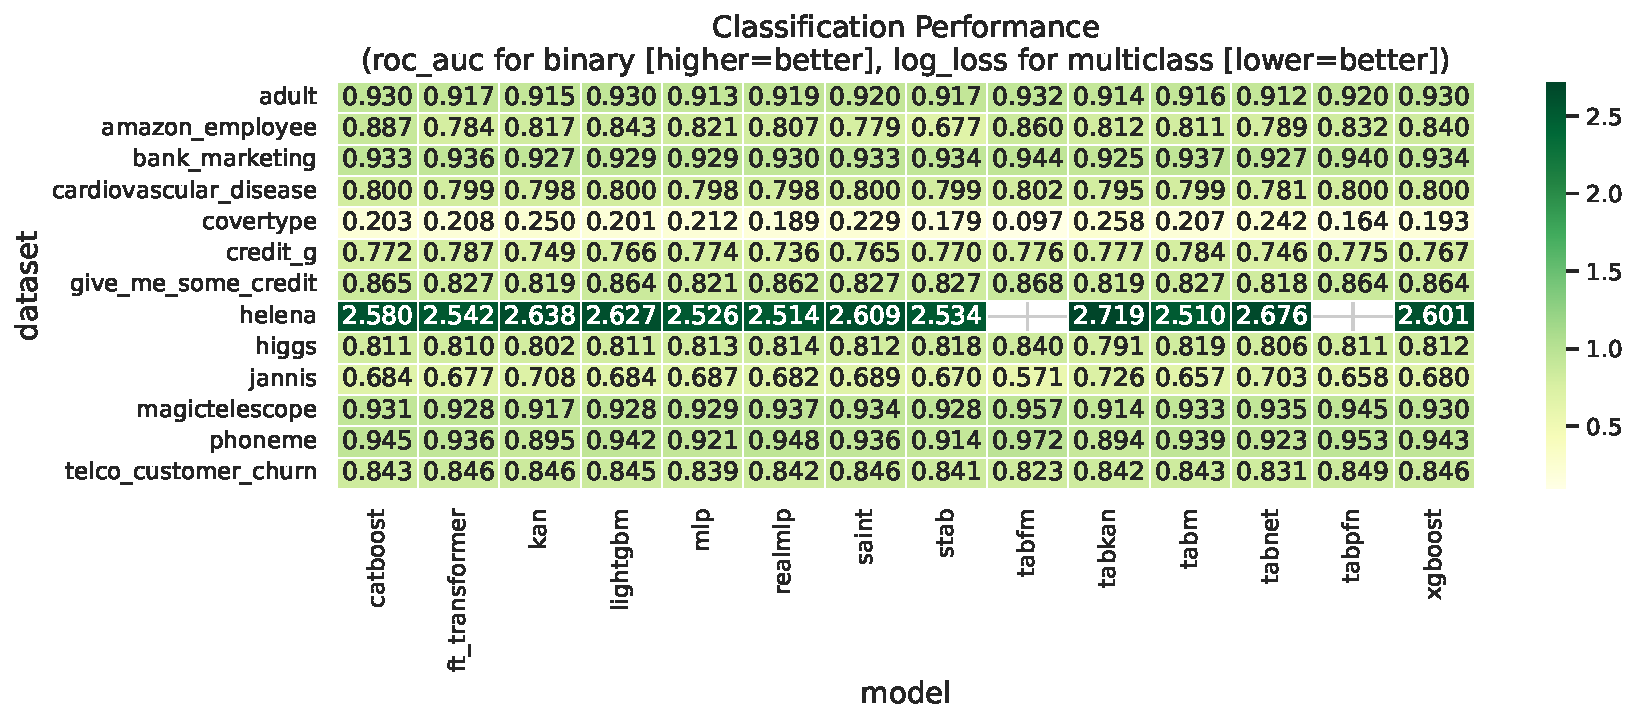
\includegraphics[width=\linewidth]{images/heatmap_classification.pdf}
\caption[Mapa de calor da classificação: métrica por modelo e
conjunto]{\textbf{As margens absolutas no topo são pequenas --- em vários
conjuntos binários, a diferença entre o melhor e a mediana dos modelos
está na segunda casa decimal de AUC.} Métrica primária por modelo
(colunas) e conjunto (linhas): ROC-AUC nas binárias (maior é melhor) e
log-loss nas multiclasse (menor é melhor) --- as duas métricas convivem
na mesma grade, de modo que a comparação válida é dentro de cada linha,
nunca entre linhas. As células vazias na linha \texttt{helena} são as
duas exclusões estruturais (TabPFN e TabFM, 100 classes acima do limite
arquitetural). Rótulos internos da figura em inglês e decimais com ponto (figura canônica do \emph{benchmark}); eixos e leitura descritos nesta legenda. Fonte:
\texttt{results/figures/heatmap\_classification.pdf}.}
\label{fig:cap5-heatmap}
\end{figure}

A leitura por conjunto confirma a do agregado --- margens pequenas no
topo das binárias --- e adiciona o que o agregado não mostra: as duas
células estruturalmente vazias ficam visíveis, e os poucos conjuntos em
que um modelo abre vantagem nítida (como o CatBoost em
\texttt{amazon\_employee}, de alta cardinalidade categórica) antecipam as
reversões condicionais do Ato~III. A ressalva permanece: valores de
\emph{hold-out} em uma única partição fixa não carregam, sozinhos, significância
--- eles ilustram; a inferência vem dos testes pareados sobre os folds.

\paragraph{O único sinal robusto do desempenho bruto está no fundo.}
Enquanto o topo empata, o fundo não: o TabNet \citep{arik2021} é
consistentemente o pior modelo da geração do núcleo, com ranks médios de
11,8 (binária), 11,7 (multiclasse) e 11,4 (regressão) na grade completa.
É o único veredito de desempenho bruto que o benchmark autoriza sem
qualificação dentro do núcleo --- e um lembrete de que arquiteturas
celebradas na literatura podem não sobreviver a um protocolo uniforme
com orçamento de ajuste equalizado.

\section{Ato II --- os eixos de custo}
\label{sec:cap5-ato2}

Se a acurácia empata, a decisão entre os modelos do topo precisa de
outros eixos --- e é neles que os modelos diferem radicalmente. Esta
seção percorre os três eixos de custo medidos pelo protocolo (tempo de
treino, custo de ajuste de hiperparâmetros e latência de inferência) e os
cruza com o desempenho na fronteira de Pareto.

\paragraph{Treino: duas ordens e meia de magnitude.}
O tempo de treino mediano varia cerca de $300\times$ dentro da grade:
LightGBM e XGBoost ajustam o modelo final em ${\sim}0{,}7$~s, enquanto
SAINT e STab consomem ${\sim}200$~s por ajuste --- e a diferença se
multiplica pelo número de tentativas de ajuste de hiperparâmetros e de
folds da validação cruzada aninhada. Os \emph{foundation models} invertem o
eixo: por serem \emph{zero-shot}, o ``treino'' do TabFM custa 0,18~s e o
do TabPFN 1,35~s, com custo de ajuste \textbf{zero} --- não há busca de
hiperparâmetros a pagar. Essa inversão, cujo outro lado aparece já no
próximo parágrafo, é o fio que costura o capítulo.

\paragraph{Ajuste de hiperparâmetros: o custo escondido.}
O segundo eixo é o custo total do ajuste de hiperparâmetros, que o tempo
de treino de um único ajuste subestima. Nas medianas entre conjuntos, os
GBDTs pagam de 106~s (LightGBM) a 648~s (CatBoost) pelo ciclo completo de
busca; o DL tipo-MLP paga de 1.150~s (MLP) a 3.515~s (TabM); e a atenção
pesada chega a 12.245~s (SAINT) e 14.956~s (STab) --- duas ordens de
magnitude acima dos GBDTs mais baratos, para, como visto no Ato~I, não
sair do empate. Os \emph{foundation models} pagam zero. Esse eixo raramente
aparece nos benchmarks da literatura, mas é o que o praticante paga a
cada reajuste do modelo em produção.

\paragraph{Inferência: cinco ordens de magnitude.}
A latência de inferência é o eixo mais dramático do benchmark. A
Figura~\ref{fig:cap5-latencia} apresenta a medição completa, feita sob
protocolo idêntico para os 14 modelos: \us{} por linha, mediana de 5
passadas sobre o \emph{hold-out} completo do \texttt{adult}, cada modelo em seu
dispositivo natural (GBDTs em CPU; modelos profundos e \emph{foundation models}
em GPU).

\begin{figure}[htbp]
\centering
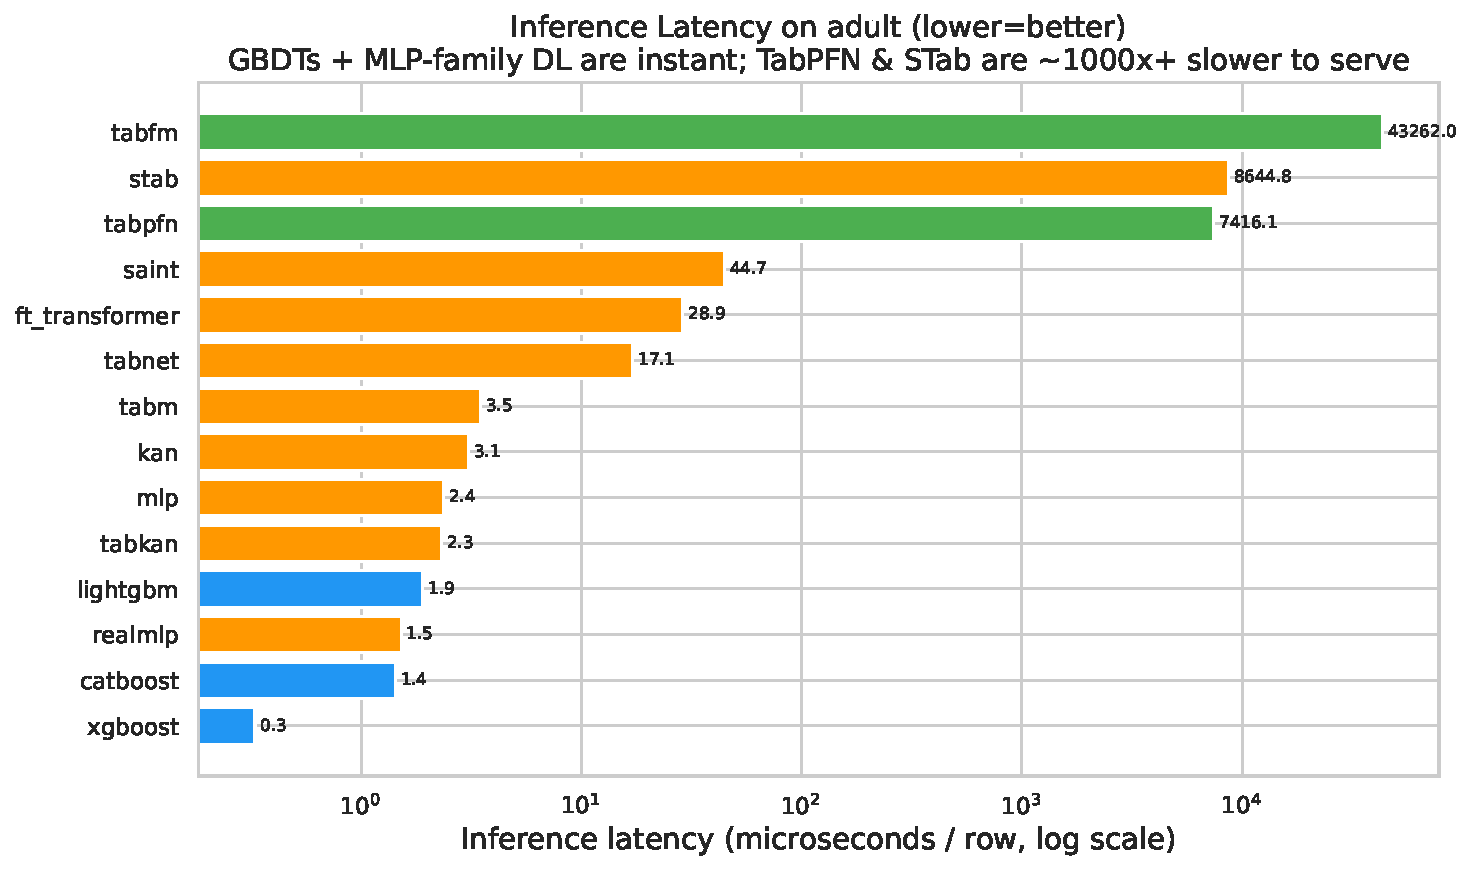
\includegraphics[width=0.95\linewidth]{images/inference_time.pdf}
\caption[Latência de inferência no \texttt{adult} (\us/linha, escala
logarítmica)]{\textbf{A latência de inferência atravessa cinco ordens de
magnitude: GBDTs e DL tipo-MLP servem em microssegundos; atenção custa
dezenas de \us; os paradigmas de inferência pesada custam milhares.}
Latência em \us{} por linha no \emph{hold-out} do \texttt{adult} (mediana de 5
passadas, escala logarítmica, menor é melhor), com cores por família.
Cada modelo roda em seu dispositivo natural (GBDTs em CPU; profundos e
\emph{foundation models} em GPU), de modo que as razões descrevem o regime de
serving em lote amortizado em uma máquina declarada --- não a latência
online de linha única, cujas diferenças são menores. Rótulos internos da figura em inglês e decimais com ponto (figura canônica do \emph{benchmark}); eixos e leitura descritos nesta legenda. Fonte:
\texttt{results/figures/inference\_time.pdf} (dados em
\texttt{results/latency/latency\_adult.csv}).}
\label{fig:cap5-latencia}
\end{figure}

A estrutura da figura organiza-se em quatro camadas. Na base, o XGBoost
serve a 0,33~\us/linha. O \emph{tier} rápido reúne os três GBDTs, os
modelos profundos tipo-MLP e as duas KANs (CatBoost 1,4; RealMLP 1,5;
LightGBM 1,9; TabKAN 2,3; MLP 2,4; KAN 3,1; TabM 3,5~\us/linha) --- um
resultado em si: aprendizado profundo \emph{não} é sinônimo de serviço
caro; a arquitetura é que decide. A atenção custa dezenas de
microssegundos (TabNet 17; FT-Transformer 29; SAINT 45). E o extremo
pertence aos paradigmas de inferência estruturalmente pesada: TabPFN
7.416, STab 8.645 e TabFM 43.262~\us/linha --- o custo do STab vem da
inferência bayesiana que calcula a média de 64 passadas estocásticas; o
dos \emph{foundation models}, de carregar o conjunto de treino como contexto a
cada predição. A ressalva de regime, dita na legenda, merece repetição
no corpo: essas razões descrevem o serviço em lote amortizado no
hardware declarado no Capítulo~\ref{chap:metodologia}; o serviço online
de linha única estreita as diferenças --- mas não as ordens de
magnitude.

\paragraph{O cruzamento: a fronteira de Pareto.}
Nenhum dos eixos isolados decide; o instrumento de decisão é o
cruzamento desempenho $\times$ custo. Sobre rank médio $\times$ custo
--- sendo o rank o instrumento primário de comparação do estudo --- o
núcleo de 11 modelos resolve-se em uma fronteira de Pareto de
\{TabPFN, XGBoost, LightGBM\} no eixo de custo de treino, que se estreita
para \{XGBoost, TabPFN\} no eixo de latência (sobre AUC média em vez de
rank, o CatBoost também entra na fronteira --- e, no eixo de latência, o
TabPFN sai dela); \textbf{todo o
aprendizado profundo clássico é dominado} em ambos os cruzamentos. A
Figura~\ref{fig:cap5-pareto} apresenta o retrato completo, já com os 14
modelos.

\begin{figure}[htbp]
\centering
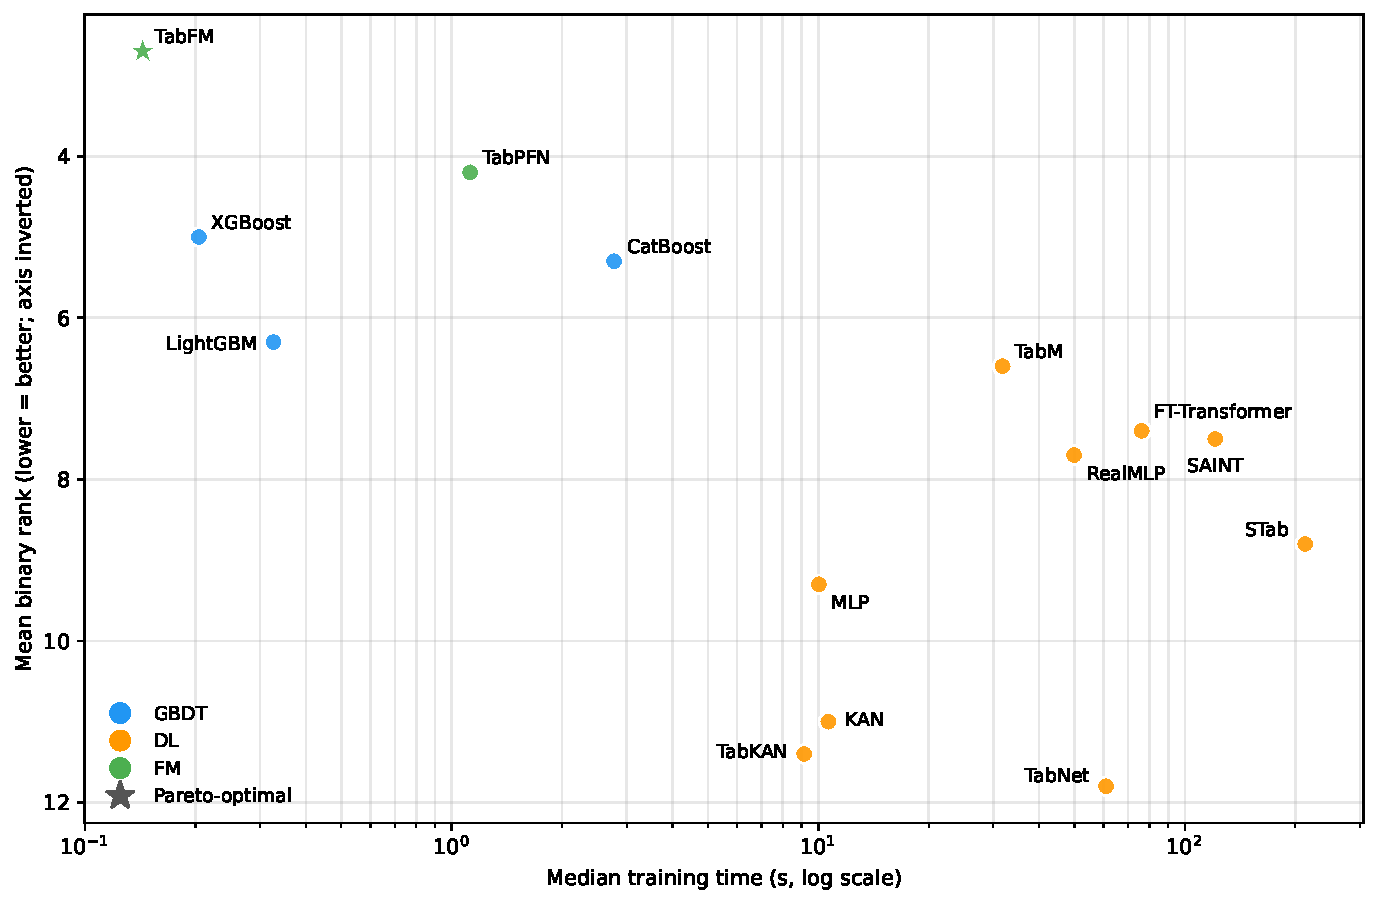
\includegraphics[width=0.92\linewidth]{images/pareto_binary.pdf}
\caption[Fronteira de Pareto: rank binário médio vs.\ tempo de
treino]{\textbf{Na grade completa, o TabFM toma a fronteira
treino-desempenho sozinho: é simultaneamente o ajuste mais barato e o
melhor rank.} Rank binário médio $\times$ tempo mediano de treino sobre
os conjuntos binários (escala logarítmica; o eixo de rank é invertido, de
modo que acima-à-esquerda é melhor), todos os 14 modelos. O ponto
estrelado é Pareto-ótimo sobre a grade completa (TabFM); a fronteira
\{TabPFN, XGBoost, LightGBM\} citada no texto é a restrição ao núcleo de
11 modelos. As comparações sobre o eixo de latência de inferência são
reportadas no texto. Rótulos internos da figura em inglês e decimais com ponto (figura canônica do \emph{benchmark}); eixos e leitura descritos nesta legenda. Fonte:
\texttt{latex/ai1/figures/pareto\_binary.pdf}.}
\label{fig:cap5-pareto}
\end{figure}

A figura mostra o que a latência isolada não mostra: no plano
treino $\times$ rank, os \emph{foundation models} ocupam o canto ótimo --- e é
só ao trocar o eixo de custo para a latência de serviço que a imagem se
inverte. Essa dupla leitura é o \textbf{achado-âncora do programa}: o
paradigma de \emph{in-context learning} compra treino de segundos e
ajuste zero ao preço de serviço proibitivo. É ela que motiva tanto o
eixo de restrições do arcabouço de decisão
(Capítulo~\ref{chap:framework}) quanto a pergunta da destilação
(Capítulo~\ref{chap:destilacao}): quanto desse preço é removível?

\achado{5.3}{Modelos praticamente equivalentes em acurácia diferem em
${\sim}300\times$ no tempo de treino e em cinco ordens de magnitude na
latência de inferência; no núcleo de 11, a fronteira de Pareto
rank~$\times$~custo é \{TabPFN, XGBoost, LightGBM\} no eixo de treino ---
e todo o aprendizado profundo clássico é dominado.}
Quando o desempenho empata, o custo decide --- e o custo não empata.

\section{Ato III --- reversões condicionais e o eixo do tamanho}
\label{sec:cap5-ato3}

O empate do Ato~I é um retrato agregado; ele não implica que todos os
problemas sejam iguais. Este ato condiciona os resultados à estrutura da
tarefa e ao tamanho amostral, e encontra reversões reais --- a matéria-prima
das perguntas de restrição do Capítulo~\ref{chap:framework}.

\paragraph{Multiclasse: o DL recente assume o topo clássico.}
Na classificação multiclasse, os modelos profundos da geração mais
recente (STab e TabM, ambos com rank médio 3,67 na grade completa) tomam
o topo clássico dos GBDTs (XGBoost, o melhor deles, fica em 6,0). A
ressalva de poder é vinculante e repetida sempre que a multiclasse
aparece: com $N{=}3$ conjuntos, a análise é \textbf{descritiva} --- não
há teste com poder útil sobre três pontos --- e por isso nenhum achado
numerado se apoia exclusivamente nela.

\paragraph{Desbalanceamento severo: vantagem relativa dos GBDTs.}
A segunda reversão aparece ao estratificar os conjuntos de classificação
pela razão de desbalanceamento. A Figura~\ref{fig:cap5-imbalance}
apresenta os ranks médios agregados por família em três faixas de
severidade.

\begin{figure}[htbp]
\centering
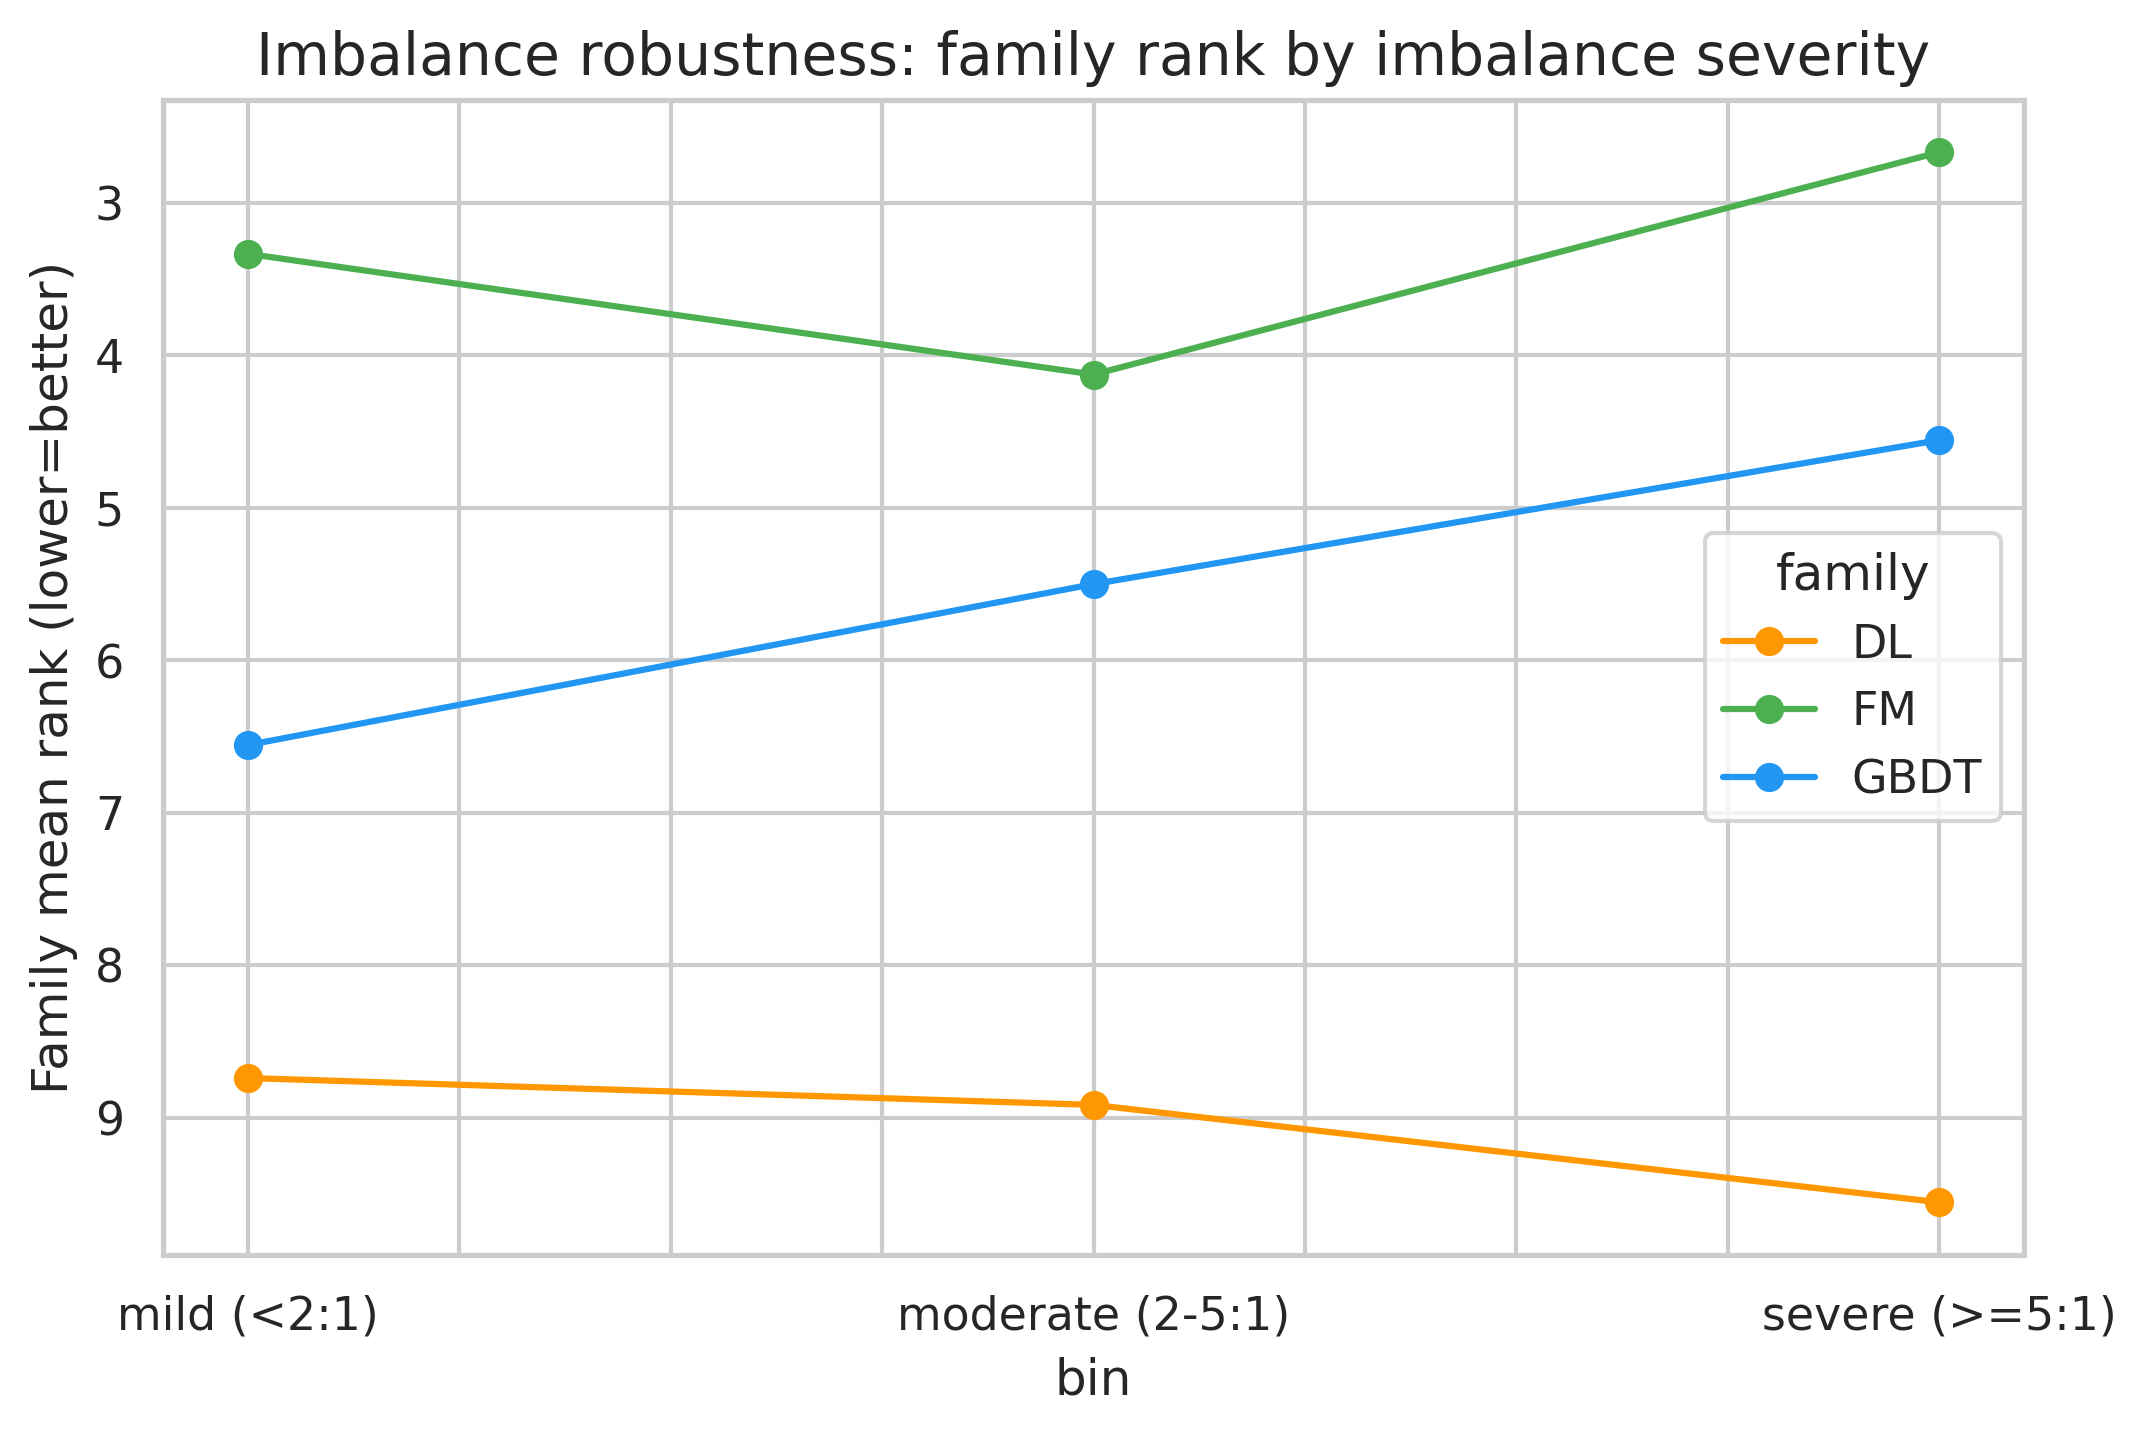
\includegraphics[width=0.85\linewidth]{images/imbalance_robustness.png}
\caption[Robustez ao desbalanceamento: rank por família e faixa de
severidade]{\textbf{Conforme o desbalanceamento se agrava, os GBDTs
melhoram seu rank relativo e o aprendizado profundo clássico piora; os
\emph{foundation models} permanecem à frente em todas as faixas.} Rank médio
agregado por família (menor é melhor; eixo invertido) nos conjuntos de
classificação, estratificados pela razão de desbalanceamento
majoritária/minoritária: leve ($<$2:1), moderada (2--5:1) e severa
($\geq$5:1). Ressalva: com poucos conjuntos por faixa, a figura é
descritiva --- ela indica direção de tendência, não significância.
Rótulos internos da figura em inglês e decimais com ponto (figura canônica do \emph{benchmark}); eixos e leitura descritos nesta legenda. O subtítulo embutido na figura (``$\sim$1000x+ slower to serve'') é um arredondamento editorial conservador da geração dela; os fatores medidos são os do texto (TabPFN 22.473$\times$, TabFM 131.097$\times$). Fonte: \texttt{results/figures/imbalance\_robustness.png}
(\texttt{notebooks/07\_segmented\_robustness.ipynb}).}
\label{fig:cap5-imbalance}
\end{figure}

A tendência é monotônica e na direção que a intuição de praticantes
sugere --- árvores lidam melhor com classes raras do que redes treinadas
por gradiente sobre perda média --- mas a ressalva da legenda é parte do
resultado: com poucos conjuntos por faixa, trata-se de direção
descritiva, não de teste. Duas observações completam o quadro
condicional: no extremo de cardinalidade categórica, a codificação
one-hot penaliza os modelos de atenção (o caso
\texttt{amazon\_employee} visível na Figura~\ref{fig:cap5-heatmap}); e o
TabPFN combina, dentro do núcleo, o melhor rank médio com o melhor
pior-caso --- é o modelo que mais raramente falha de forma catastrófica,
um atributo de robustez que rank médio sozinho não captura.

\paragraph{O eixo do tamanho: curvas de aprendizado.}
Nenhuma das análises anteriores responde à pergunta mais frequente do
praticante: ``com \emph{meu} volume de dados, quem vence?''. As curvas
de aprendizado --- 6 modelos $\times$ 5 conjuntos $\times$ 3 sementes,
varrendo de 500 amostras ao \emph{pool} completo --- dão forma a esse eixo. A
Figura~\ref{fig:cap5-curvas} apresenta a varredura completa.

\begin{figure}[htbp]
\centering
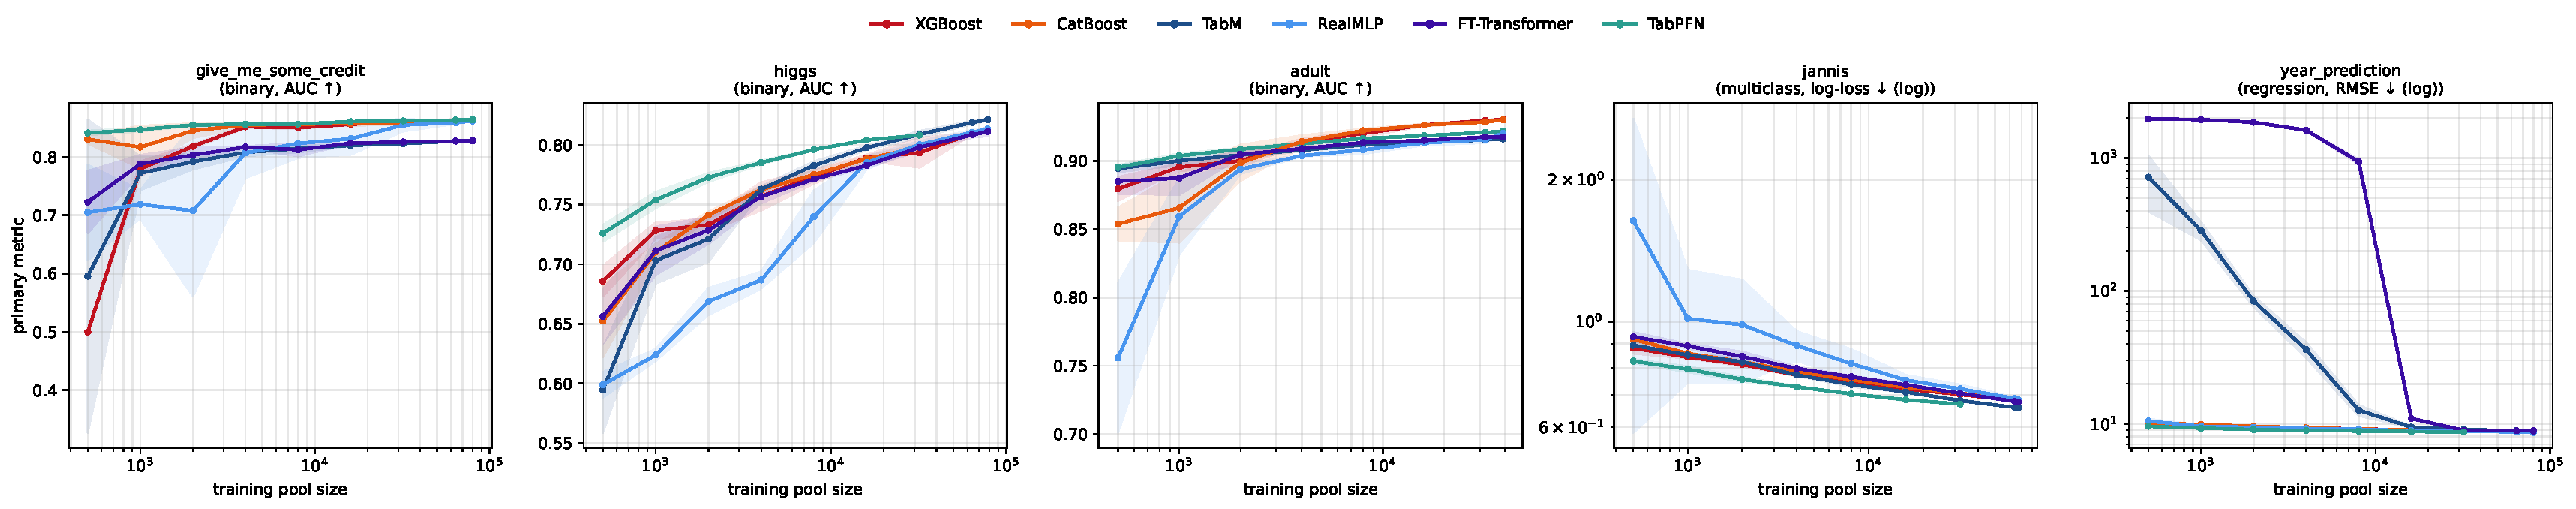
\includegraphics[width=\linewidth]{images/learning_curves.pdf}
\caption[Curvas de aprendizado: 6 modelos, 5 conjuntos, 500 amostras ao
pool completo]{\textbf{O cruzamento de liderança GBDT$\leftrightarrow$DL
é real, mas específico por conjunto --- e o TabPFN lidera o regime de
poucos dados em todos os cinco painéis.} Curvas de aprendizado (6
modelos $\times$ 5 conjuntos $\times$ 3 sementes, de 500 amostras ao \emph{pool}
completo). Cada painel nomeia sua métrica e direção ($\uparrow$ maior é
melhor; $\downarrow$ menor, escala logarítmica); as bandas são $\pm$1
desvio-padrão sobre as sementes. Um cruzamento é o ponto em que a curva
de uma família cruza permanentemente a da outra. Rótulos internos da figura em inglês e decimais com ponto (figura canônica do \emph{benchmark}); eixos e leitura descritos nesta legenda. Fonte:
\texttt{latex/ai1/figures/learning\_curves.pdf}
(\texttt{notebooks/10\_learning\_curves.ipynb}).}
\label{fig:cap5-curvas}
\end{figure}

Três leituras saem da figura. Primeira: o cruzamento de liderança entre
GBDTs e DL existe, mas é específico por conjunto --- em 3 dos 5
conjuntos varridos (\texttt{higgs}, \texttt{jannis} e
\texttt{year\_prediction}), o DL ultrapassa os GBDTs e não devolve a
liderança; no \texttt{adult}, o GBDT a retoma em $n \approx 4.000$; e em
\texttt{give\_me\_some\_credit}, o GBDT lidera do início ao fim. Não há,
portanto, um ``$n$ crítico'' universal a recomendar: a resposta honesta
ao praticante é que o cruzamento depende do conjunto, não apenas do
tamanho. Segunda: o TabPFN
tem a melhor métrica média de regime nos cinco conjuntos varridos para
$n \leq 4.000$ (rank médio 1,0 nesse regime, contra 2,8 do XGBoost) ---
a quantificação do nicho de poucos dados do paradigma \emph{zero-shot}.
Terceira, a ressalva: a varredura cobre 6 dos 14 modelos e 5 dos 18
conjuntos; ela qualifica o eixo do tamanho, não o reordena.

\achado{5.4}{A melhor família depende da estrutura do problema --- o DL
recente toma o topo multiclasse (descritivo), os GBDTs ganham vantagem
relativa sob desbalanceamento severo, o one-hot penaliza a atenção no
extremo categórico --- e o cruzamento GBDT$\leftrightarrow$DL por
tamanho é real mas específico por conjunto, com o TabPFN dominando o
regime $n \leq 4.000$ em todos os conjuntos varridos.}
As reversões não restauram a máxima de uma família vencedora: elas
mostram que a resposta certa é condicional --- e condições verificáveis
a priori são exatamente o que um arcabouço de decisão pode codificar.

\section{Ato IV --- a quebra do empate: a geração 2026}
\label{sec:cap5-ato4}

\paragraph{A entrada do TabFM reorganiza a narrativa.}
A expansão para a grade completa de 14 modelos muda o retrato. O TabFM
--- \emph{foundation model} lançado em junho de 2026, avaliado aqui
\emph{zero-shot}, sem qualquer ajuste por conjunto --- lidera o rank
médio \textbf{nas três tarefas}: 2,7 na binária, 1,0 na multiclasse
(pontuação perfeita sobre seus dois conjuntos elegíveis;
\texttt{helena} é exclusão estrutural) e 1,2 na regressão. É o melhor
modelo absoluto em \textbf{13 dos 18 conjuntos}, participando de 17. A
Tabela~\ref{tab:cap5-ranks} resume os ranks por tarefa e a
Figura~\ref{fig:cap5-ranks} apresenta o retrato visual.

\begin{table}[htbp]
\centering
\caption[Rank médio por tarefa --- geração 2026 vs.\ referências]{Rank
médio por tarefa --- geração 2026 vs.\ referências ($k{=}14$ modelos;
binária $N{=}10$, multiclasse $N{=}3$, regressão $N{=}5$; menor é melhor,
\textbf{negrito} = melhor da coluna). Os ranks multiclasse de TabFM e
TabPFN são médias sobre os 2 conjuntos excluindo \texttt{helena}
(exclusão estrutural). A tabela mestra completa, com a métrica primária
de cada modelo em cada um dos 18 conjuntos, está no
Apêndice~\ref{app:tabelas}. Fonte:
\texttt{notebooks/TABELA\_RESULTADOS.md}.}
\label{tab:cap5-ranks}
\begin{tabular}{lccc}
\toprule
 & Binária & Multiclasse & Regressão \\
\midrule
\textbf{TabFM}      & \textbf{2,7} & \textbf{1,00} & \textbf{1,2} \\
TabPFN              & 4,2          & 2,50          & 3,0 \\
Melhor clássico     & XGBoost 5,0  & STab/TabM 3,67 & XGBoost 5,0 \\
KAN                 & 11,0         & 12,0          & 9,8 \\
TabKAN              & 11,4         & 13,3          & 11,8 \\
\bottomrule
\end{tabular}
\end{table}

\begin{figure}[htbp]
\centering
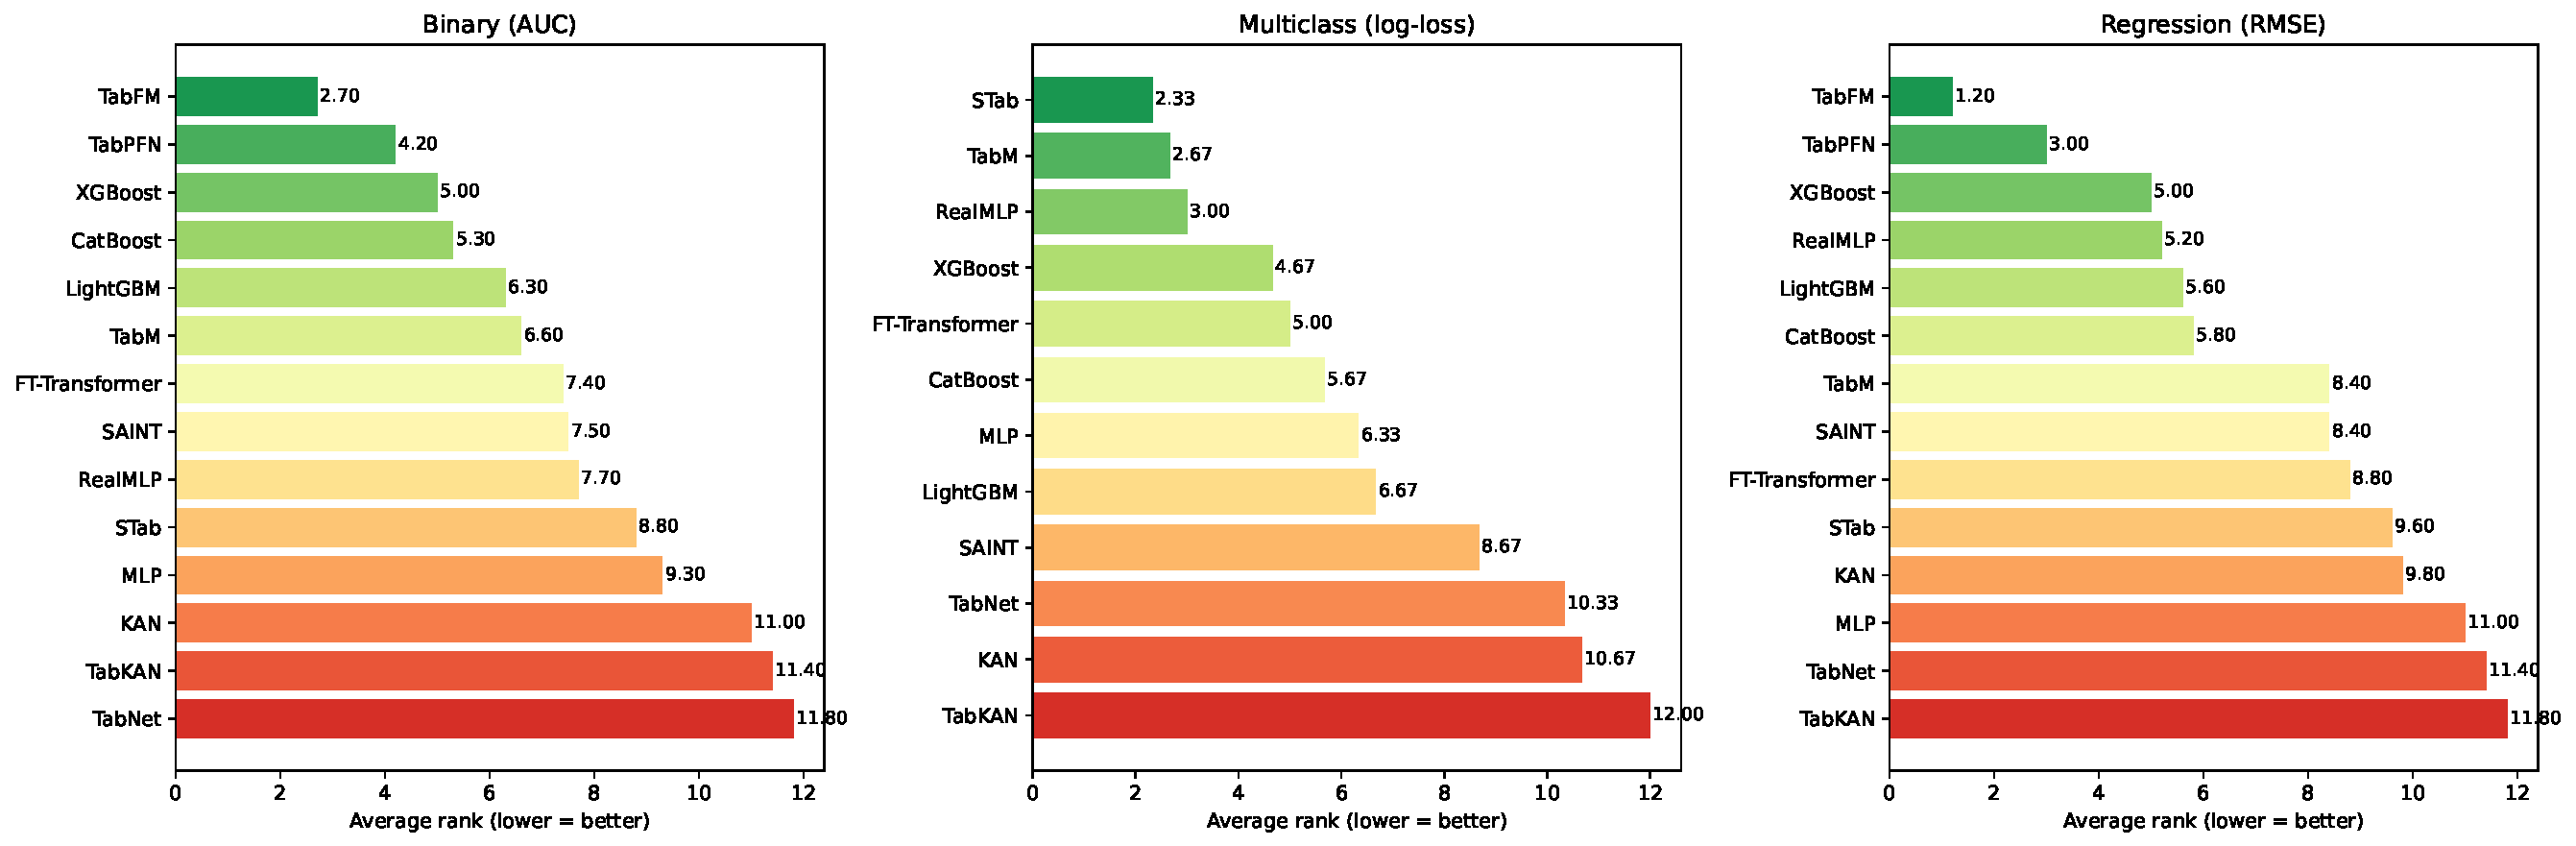
\includegraphics[width=0.92\linewidth]{images/average_ranks.pdf}
\caption[Ranks médios por tarefa, grade completa]{\textbf{A geração 2026
(TabFM) separa-se do pelotão nos painéis de binária e regressão; as KANs
ocupam o último terço em todos.} Ranks médios por tarefa. Os painéis de
binária e regressão cobrem os 14 modelos; o painel multiclasse mostra os
12 modelos avaliados nos três conjuntos multiclasse, rankeados dentro
desse subconjunto --- e por isso não é diretamente comparável aos ranks
de 14 modelos da Tabela~\ref{tab:cap5-ranks}, em que os foundation
models (excluídos no \texttt{helena}) são rankeados. Rótulos internos da figura em inglês e decimais com ponto (figura canônica do \emph{benchmark}); eixos e leitura descritos nesta legenda. Fonte:
\texttt{latex/ai1/figures/average\_ranks.pdf}.}
\label{fig:cap5-ranks}
\end{figure}

Dois detalhes concretos dão escala à liderança. Na multiclasse, onde a
margem é mais visível, o TabFM alcança log-loss de 0,0966 no
\texttt{covertype} e 0,5709 no \texttt{jannis}, contra 0,1644 e 0,6583
do segundo colocado (TabPFN) --- margens visivelmente maiores que as que
separam vizinhos de rank dentro do núcleo de 11 na mesma tabela
(Apêndice~\ref{app:tabelas}). E o TabPFN, por sua vez,
consolida-se como o vice consistente da grade (ranks médios
4,2/2,5/3,0 nas três tarefas): a geração 2026 não é um ponto fora da
curva, é uma família inteira --- os dois \emph{foundation models} ocupam os
dois primeiros postos em todas as tarefas.

A consequência interpretativa é a re-escopagem do Ato~I: o empate fica
corretamente lido como \emph{retrato da geração anterior}. Não foi o
aprendizado profundo ajustado que alcançou os GBDTs; foi o pré-treino que
atropelou ambos. E a cautela estatística permanece dita: com $k{=}14$ e
$N{=}10$, a distância crítica de Nemenyi é larga
(Figura~\ref{fig:cap5-cd}) --- a separação do TabFM apoia-se na
consistência entre conjuntos (13 vitórias em 18) e no instrumento
bayesiano, \textbf{não} no post-hoc frequentista. Duas condições de
contorno adicionais são declaradas: na regressão, $N{=}5$ põe o piso do
p-valor de Wilcoxon em 0,0625 (piso combinatório --- nenhum resultado
pode ser ``significativo a 5\%'' ali); e o TabFM é avaliado na versão
fixada v1.0.1 (julho de 2026), cujo relatório técnico oficial apareceu
apenas no fim de setembro de 2026 \citep{kong2026} e segue sem revisão
por pares --- os resultados são sobre essa versão, e isso fica
registrado.

\paragraph{O contrapeso: o líder de acurácia é o pior em latência.}
O contrapeso é frontal, e é o achado-âncora do programa: o líder de
acurácia é o pior modelo da grade em latência de serviço ---
43.262~\us/linha sob o protocolo padrão, $131.097\times$ o XGBoost, e
mais em contextos maiores, chegando a ${\sim}394$~ms/linha no maior
conjunto de regressão. A pergunta de decisão mudou de natureza: não é
mais ``qual família vence?'', e sim ``\emph{a latência do foundation
model cabe no caso de uso?}''.

\achado{5.5}{A geração 2026 quebra o empate: o TabFM lidera o rank médio
nas três tarefas e é o melhor modelo em 13 dos 18 conjuntos, \emph{zero-shot}
--- ao preço de quatro a cinco ordens de magnitude em latência de
serving (43.262 vs.\ 0,33~\us/linha).}
O empate não tornou o arcabouço multicritério obsoleto; a quebra o
tornou mais necessário --- e apontou seu único obstáculo.

\paragraph{O resultado negativo das redes de Kolmogorov--Arnold.}
No mesmo movimento da extensão, o benchmark produz o teste independente
da família Kolmogorov--Arnold --- e o resultado é o negativo de valor.
KAN (ranks 11,0/12,0/9,8 em binária/multiclasse/regressão) e TabKAN
(11,4/13,3/11,8) ocupam o último terço nas três tarefas, com o TabKAN
atrás até do TabNet em multiclasse e regressão. Surpreendente à luz das
alegações dos artigos originais \citep{kan2024,tabkan2025}, o resultado
pede explicação: sob protocolo uniforme com orçamento de ajuste
equalizado, as alegações não se sustentam, e a explicação mais provável
é que as comparações originais usaram \emph{baselines} subajustados ---
leitura consistente com a literatura cética anterior
\citep{poeta2024,kancritical2024}. Até onde alcança nossa verificação
datada de novidade, este é o primeiro teste da família contra a grade
completa GBDT/DL/foundation-model em um benchmark tabular multicritério;
as avaliações independentes anteriores
\citep{poeta2024,kancritical2024} comparam KANs apenas contra MLPs e não
medem eixos de custo. A contraparte de engenharia merece registro
simétrico: ambas habitam o \emph{tier} rápido de latência (2,3--3,1~\us/linha)
e custam VRAM desprezível --- \textbf{o problema é o desempenho, não o
custo}.

\achado{5.6}{Sob protocolo uniforme, KAN e TabKAN ficam no último terço
nas três tarefas --- as alegações dos artigos originais não se
sustentam no primeiro teste independente contra a grade completa, até
onde alcança nossa verificação datada --- embora ambas sejam baratas de
servir.}
O resultado negativo é reportado com o mesmo estatuto dos positivos,
conforme o contrato de conduta do estudo
(Capítulo~\ref{chap:metodologia}): um benchmark neutro existe
precisamente para que resultados assim venham a público.

\section{Síntese do capítulo}
\label{sec:cap5-sintese}

Três fatos encadeados emergem do benchmark. \textbf{(i)}~Na geração do
núcleo de 11 modelos, o desempenho bruto empata no topo --- empate
positivo, aferido por equivalência prática bayesiana e robusto à
variação do limiar --- e 80\% da variância de rank é intrafamília; a
decisão racional migra, portanto, para custo, latência, robustez e
estrutura da tarefa, exatamente os eixos em que os modelos diferem por
ordens de magnitude. \textbf{(ii)}~A geração 2026 quebra o empate em
acurácia: o TabFM lidera as três tarefas e vence em 13 de 18 conjuntos,
\emph{zero-shot} --- ao preço de quatro a cinco ordens de magnitude em latência
de serving, invertendo o eixo de custo (treino de segundos e ajuste
zero; serviço proibitivo). A quebra não aposenta a leitura
multicritério: ela a torna mais necessária, porque a escolha ótima
passa a depender de uma única restrição dominante. \textbf{(iii)}~Essa
restrição é atacável: a latência do \emph{foundation model} não é uma lei, é um
custo de arquitetura --- e custos de arquitetura podem ser transferidos
para modelos pequenos. As ressalvas do capítulo acompanham os fatos:
$N$ pequeno por tarefa (multiclasse descritiva; piso de p-valor na
regressão), distância crítica larga na grade completa, latências medidas
no regime de lote amortizado em dispositivo natural, e TabFM avaliado em
versão fixada anterior à revisão por pares de seu relatório técnico.

\begin{transicao}
O Capítulo~\ref{chap:framework} converte o fato (i) e as reversões do
Ato~III em um arcabouço de decisão por restrições --- e o valida por
\emph{leave-one-dataset-out}, testando tanto a alternativa de roteamento
por meta-características (resultado negativo) quanto a política fixa
``\emph{foundation model} primeiro, desviar por restrições'' (resultado
positivo). O obstáculo que resta a essa política --- as quatro a cinco
ordens de magnitude de latência do fato (ii) --- é o objeto do
Capítulo~\ref{chap:destilacao}: quanto dele a destilação remove, e sob
quais condições verificáveis.
\end{transicao}
